\documentclass{beamer}

\usefonttheme{professionalfonts} % using non standard fonts for beamer
\usefonttheme{serif} % default family is serif

\usepackage{hyperref}

\usepackage{animate}

\usepackage{graphicx}

\def\Put(#1,#2)#3{\leavevmode\makebox(0,0){\put(#1,#2){#3}}}

\usepackage{color}

\usepackage{tikz}

\usepackage{amssymb}

\usepackage{enumerate}



\newcommand\blfootnote[1]{%

  \begingroup

  \renewcommand\thefootnote{}\footnote{#1}%

  \addtocounter{footnote}{-1}%

  \endgroup

}

\makeatletter

%%%%%%%%%%%%%%%%%%%%%%%%%%%%%% Textclass specific LaTeX commands.

 % this default might be overridden by plain title style

 \newcommand\makebeamertitle{\frame{\maketitle}}%

 % (ERT) argument for the TOC

 \AtBeginDocument{%

   \let\origtableofcontents=\tableofcontents

   \def\tableofcontents{\@ifnextchar[{\origtableofcontents}{\gobbletableofcontents}}

   \def\gobbletableofcontents#1{\origtableofcontents}

 }

%%%%%%%%%%%%%%%%%%%%%%%%%%%%%% User specified LaTeX commands.

\usetheme{Malmoe}

% or ...

\useoutertheme{infolines}

\addtobeamertemplate{headline}{}{\vskip2pt}


\setbeamertemplate{theorems}[numbered]
\setbeamercovered{transparent}
\theoremstyle{definition}
\newtheorem{defn}{Definition}[section]

% or whatever (possibly just delete it)

\makeatother

\begin{document}
\title[Discussion 02]{CS/MATH 111, Discrete Structures - Fall 2018. \\ Discussion 02 - Proof by Induction, Logarithms, Asymptotic Notation and Execution Time.}
\author[CS111]{Andres, Sara, Elena}
\institute[Winter'19]{University of California, Riverside}
\makebeamertitle
\newif\iflattersubsect

\AtBeginSection[] {
    \begin{frame}<beamer>
    \frametitle{Outline} 
    \tableofcontents[currentsection]  
    \end{frame}
    \lattersubsectfalse
}

\AtBeginSubsection[] {
    \begin{frame}<beamer>
    \frametitle{Outline} 
    \tableofcontents[currentsubsection]  
    \end{frame}
}

\section{Proof by induction}

\begin{frame}{Example 1}
Use mathematical induction to show that 
$$ 1 + 2 + 2^2 + \cdots + 2^n = 2^{n + 1} - 1 $$
for all nonnegative integers $n$.

    \begin{enumerate}[<+->]
        \item \textbf{Basis step:} For $n = 0$, $2^0 = 1 = 2^1 - 1$ is true!
        \item \textbf{Assumption step:} Let $n = k$, so $$ 1 + 2 + 2^2 + \cdots + 2^k = 2^{k + 1} - 1 $$ holds...
        \item \textbf{Inductive step:} Let's solve for $n = k + 1$,
        $$ 1 + 2 + 2^2 + \cdots + 2^{k + 1} = 2^{(k + 1) + 1} - 1 $$
    \end{enumerate}
\end{frame}

\begin{frame}{Example 1}
    \begin{enumerate}
        \item[3] \textbf{Inductive step:} Let's solve for $n = k + 1$,
        { \small 
            \uncover<+->{$$ 1 + 2 + 2^2 + \cdots + 2^{k + 1} \stackrel{?}{=} 2^{(k + 1) + 1} - 1 $$ }
            \uncover<+->{$$ 1 + 2 + 2^2 + \cdots + 2^k + 2^{k + 1} \stackrel{?}{=} 2^{k + 2} - 1 $$ }
            \uncover<+->{$$ 2^{k + 1} - 1 + 2^{k + 1} \stackrel{?}{=} 2^{k + 2} - 1 $$ }
            \uncover<+->{$$ 2 \cdot 2^{k + 1} - 1 \stackrel{?}{=} 2^{k + 2} - 1 $$ }
            \uncover<+->{$$ 2^{k + 2} - 1 = 2^{k + 2} - 1 $$ }
        }
    \end{enumerate}
\end{frame}

\begin{frame}{Example 2}
Prove the following statement by induction:
$$ 1 + 2^2 + 3^2 + \cdots + n^2 = \frac{n \cdot (n + 1) \cdot (2n + 1)}{6} $$
    \begin{enumerate}[<+->]
        \item \textbf{Basis step:} For $n = 1$, $1 = \frac {1 \times 2 \times 3}{6}$ is true!
        \item \textbf{Assumption step:} Let $n = k$, so $$ 1 + 2^2 + 3^2 + \cdots + k^2 = \frac{k \cdot (k + 1) \cdot (2k + 1)}{6} $$ holds...
        \item \textbf{Inductive step:} Let's solve for $n = k + 1$,
        $$ 1 + 2^2 + 3^2 + \cdots + (k + 1)^2 = \frac{(k + 1) \cdot ((k + 1) + 1) \cdot (2 \cdot (k + 1) + 1)}{6} $$
    \end{enumerate}
\end{frame}

\begin{frame}{Example 2}
    \begin{enumerate}
        \item[3] \textbf{Inductive step:} Let's solve for $n = k + 1$,
        { \small
            \uncover<+->{$$ 1 + 2^2 + 3^2 + \cdots + (k + 1)^2 \stackrel{?}{=} \frac{(k + 1) \cdot ((k + 1) + 1) \cdot (2 \cdot (k + 1) + 1)}{6} $$ }
            \uncover<+->{$$ 1 + 2^2 + 3^2 + \cdots + k^2 + (k + 1)^2 \stackrel{?}{=} \frac{(k + 1) \cdot (k + 2) \cdot (2k + 2 + 1)}{6} $$ }
            \uncover<+->{$$ \frac{k \cdot (k + 1) \cdot (2k + 1)}{6} + (k + 1)^2 \stackrel{?}{=} \frac{(k + 1) \cdot (k + 2) \cdot (2k + 3)}{6} $$ }
            \uncover<+->{$$ \frac{k \cdot (k + 1) \cdot (2k + 1) + 6(k + 1)^2}{6} \stackrel{?}{=} \frac{(k + 1) \cdot (k + 2) \cdot (2k + 3)}{6} $$ }
            \uncover<+->{$$ (k + 1) \cdot (k \cdot (2k + 1) + 6(k + 1)) \stackrel{?}{=} (k + 1) \cdot (k + 2) \cdot (2k + 3) $$ }
            \uncover<+->{$$ (k + 1) \cdot (2k^2 + 7k + 6) \stackrel{?}{=} (k + 1) \cdot (k + 2) \cdot (2k + 3) $$ }
            \uncover<+->{$$ (k + 1) \cdot (k + 2) \cdot (2k + 3) = (k + 1) \cdot (k + 2) \cdot (2k + 3) $$ }
        }
    \end{enumerate}
\end{frame}

\section{Logarithms}

\begin{frame}{Exponential functions}
    \centering 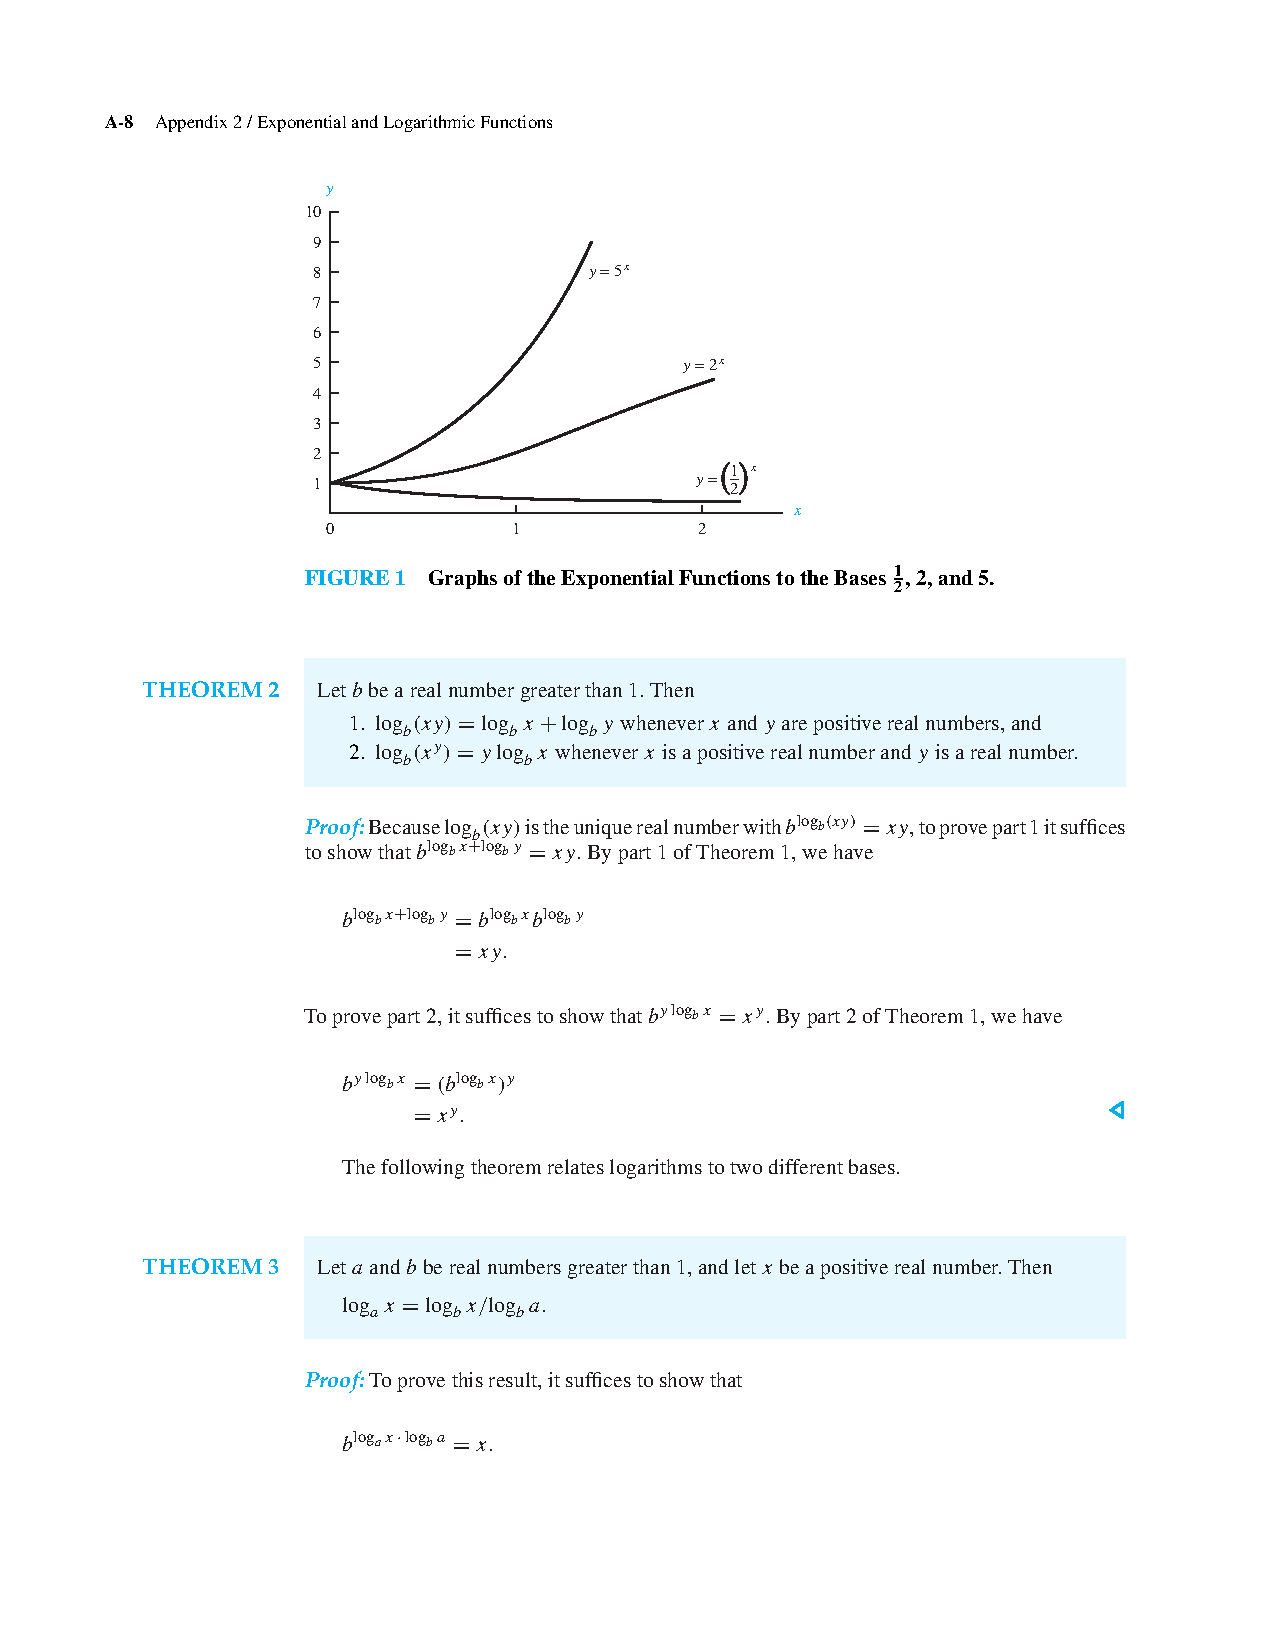
\includegraphics[trim={2cm 18.5cm 4cm 3cm},clip,width=\linewidth]{a-8}
\end{frame}

\begin{frame}{Logarithmic functions}
    \centering 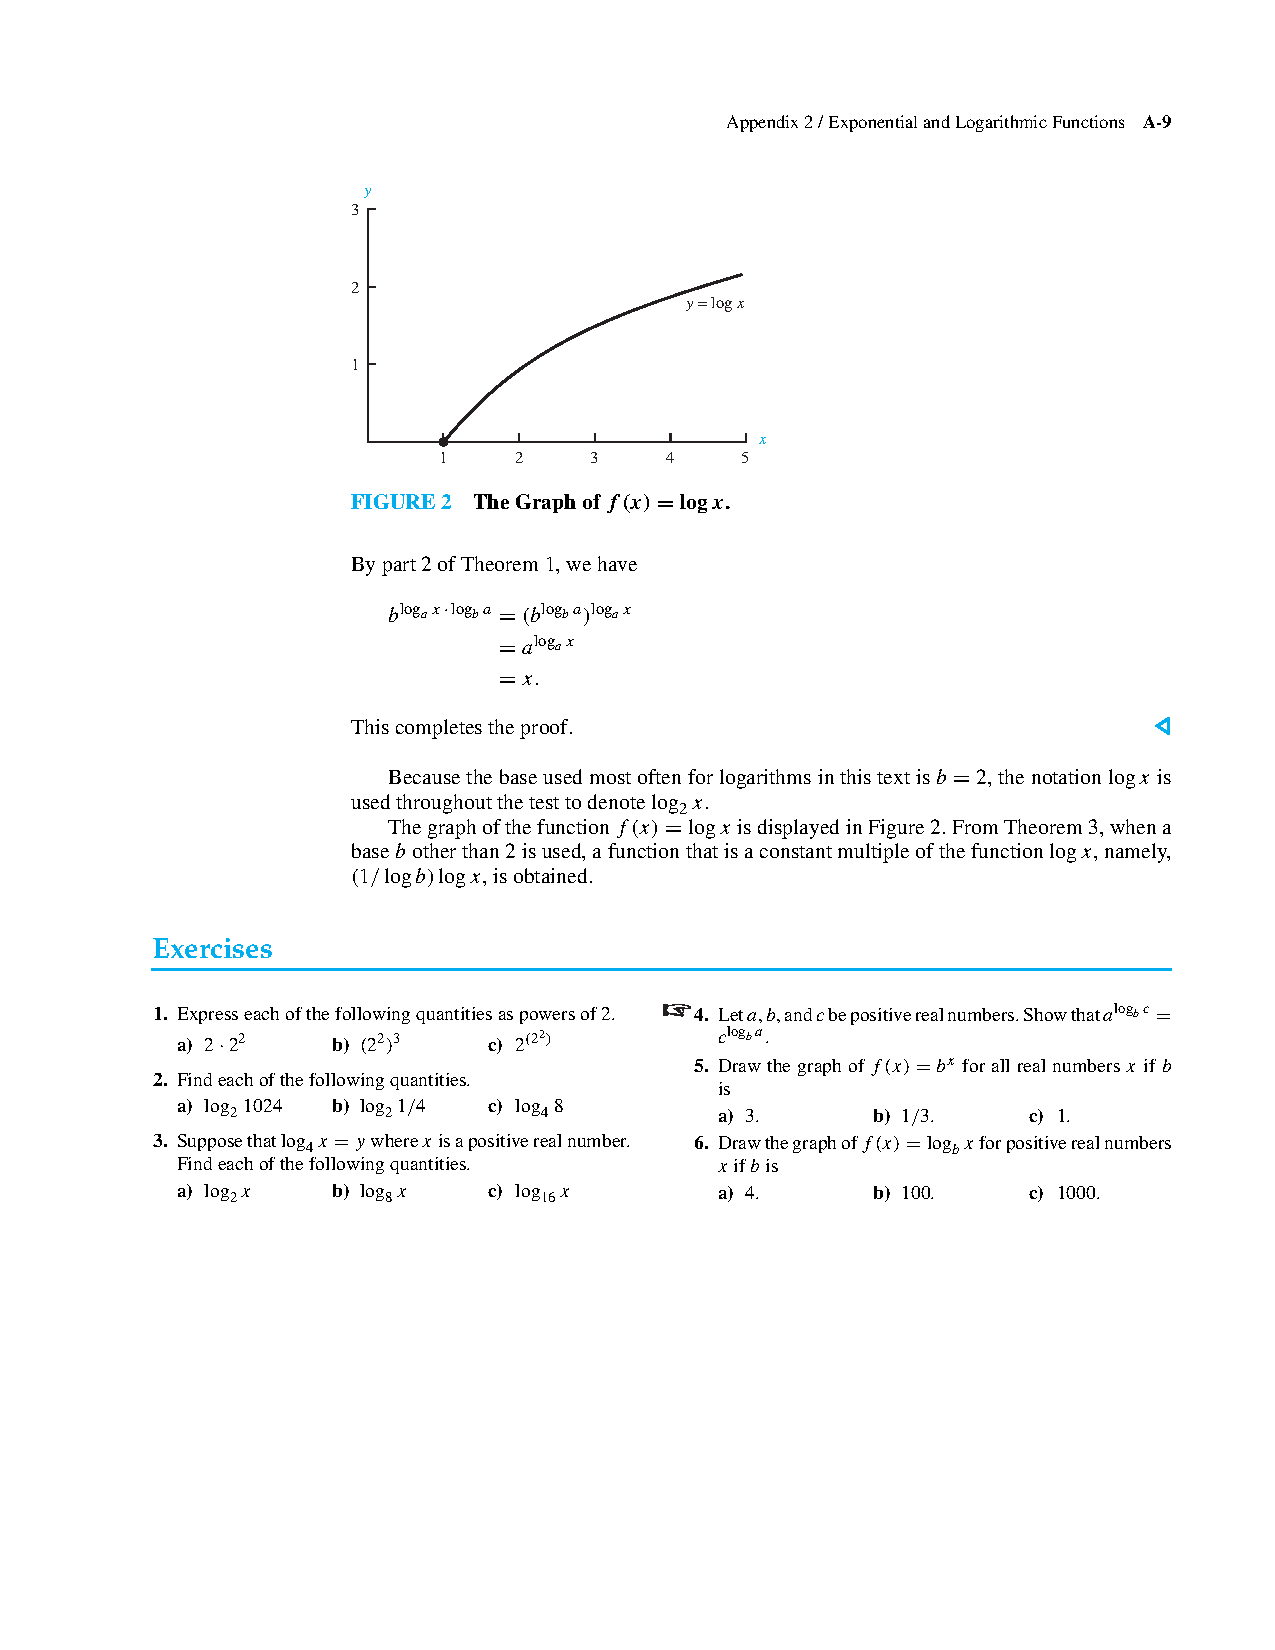
\includegraphics[trim={2cm 20cm 4cm 3cm},clip,width=\linewidth]{a-9}
\end{frame}

\begin{frame}{Theorems}
    \begin{theorem}\label{theo:one}
        Let $b$ be a positive real number and $x$ and $y$ real numbers. Then,
        \begin{enumerate}
         \item $b^{x+y} = b^x \cdot b^y$, and
         \item $(b^x)^y = b^{x \cdot y}$.
        \end{enumerate}
    \end{theorem}

\end{frame}

\begin{frame}{Theorems}
    \begin{theorem}\label{theo:two}
        Let $b$ be a real number greater than 1. Then,
        \begin{enumerate}
         \item $\log_b (xy) = \log_b x + \log_b y$ whenever $x$ and $y$ are positive real numbers, and
         \item $\log_b (x^y) = y \log_b x$ whenever $x$ is a positive real number and $y$ is a real number.
        \end{enumerate}
    \end{theorem}
\end{frame}

\begin{frame}{Theorems}
    \begin{theorem}\label{theo:three}
        Let $a$ and $b$ be real numbers greater than 1, and let $x$ be a positive real number. Then,
        \begin{enumerate}
         \item $\log_a x = \frac{\log_b x}{\log_b a}$.
        \end{enumerate}
    \end{theorem}
\end{frame}

\section{Asymptotic notation}

\begin{frame}{Big-$\mathcal{O}$ notation}
    \begin{defn}
        Let $f$ and $g$ be functions from the set of integers or the set of real numbers to the set of real numbers. We say that $f(x)$ is $\mathcal{O}(g(x))$ if there are constants $C$ and $k$ such that,
        $$ |f(x)| \leq C|g(x)| $$
        whenever $x > k$. [This is read as ``$f(x)$ is big-oh of $g(x)$.'']
    \end{defn}
\end{frame}

\begin{frame}{Big-$\Omega$ notation}
    \begin{defn}
        Let $f$ and $g$ be functions from the set of integers or the set of real numbers to the set of real numbers. We say that $f(x)$ is $\Omega(g(x))$ if there are positive constants $C$ and $k$ such that,
        $$ |f(x)| \geq C|g(x)| $$
        whenever $x > k$. [This is read as ``$f(x)$ is big-omega of $g(x)$.'']
    \end{defn}
\end{frame}

\begin{frame}{Big-$\Theta$ notation}
    \begin{defn}
        Let $f$ and $g$ be functions from the set of integers or the set of real numbers to the set of real numbers. We say that $f(x)$ is $\Theta(g(x))$ if $f(x)$ is $\mathcal{O}(g(x))$ and $f(x)$ is $\Omega(g(x))$. \\
        Also note that $f(x)$ is $\Theta(g(x))$ iif there are real numbers $C_1$ and $C_2$ and a positive real number $k$ such that,
        $$ C_1 |g(x)| \leq |f(x)| \leq C_2 |g(x)| $$
        whenever $x > k$. [This is read as ``$f(x)$ is big-theta of $g(x)$.'']
    \end{defn}
\end{frame}

\begin{frame}{Asymptotic notation \footnote{Great additional resources at \url{https://tinyurl.com/o5lwvgp}}}
    \centering 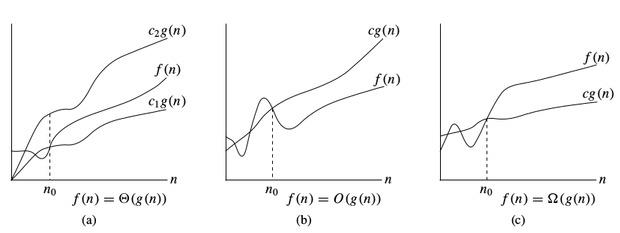
\includegraphics[width=0.8\linewidth]{notations}
\end{frame}

\section{Execution time}

\begin{frame}{Growth of functions}
    \centering 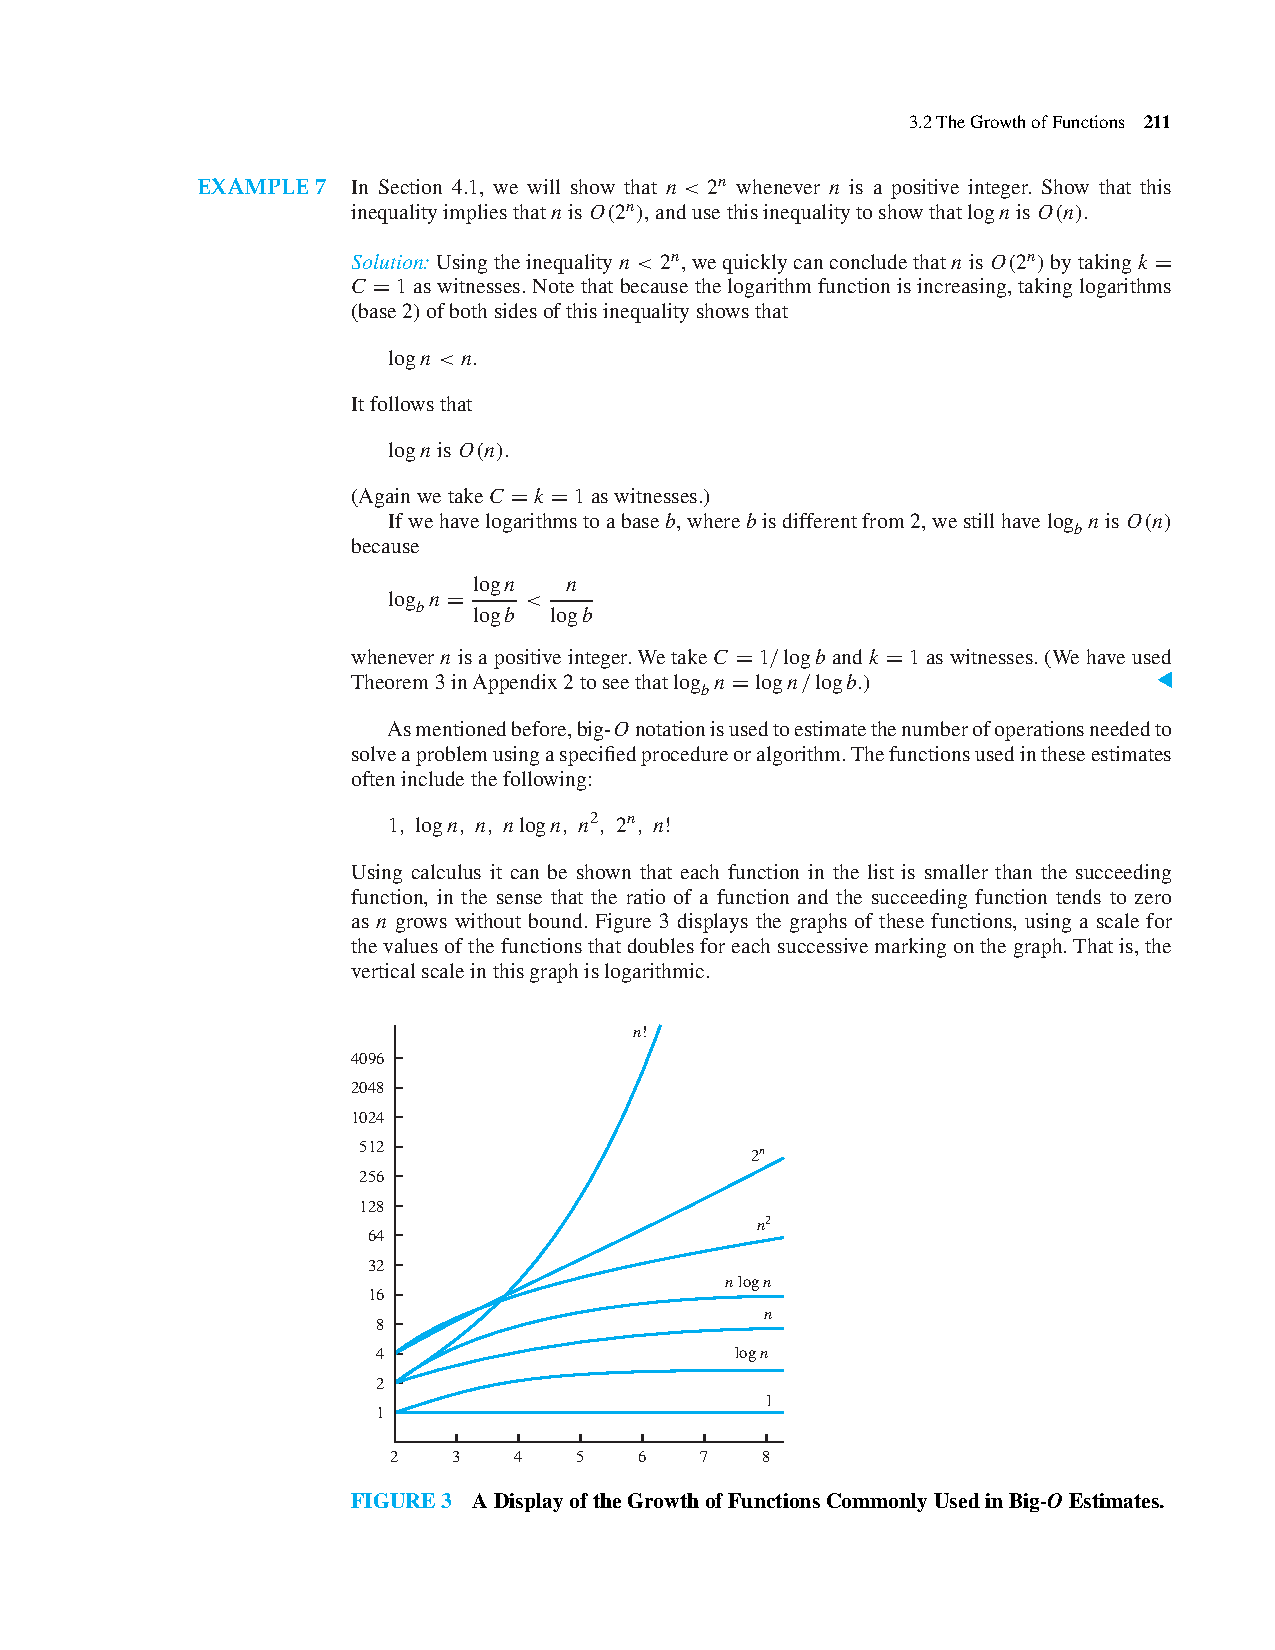
\includegraphics[trim={2cm 3cm 6cm 17cm},clip,width=\linewidth]{p211}
\end{frame}

\begin{frame}{Complexity of algorithms}
    \centering 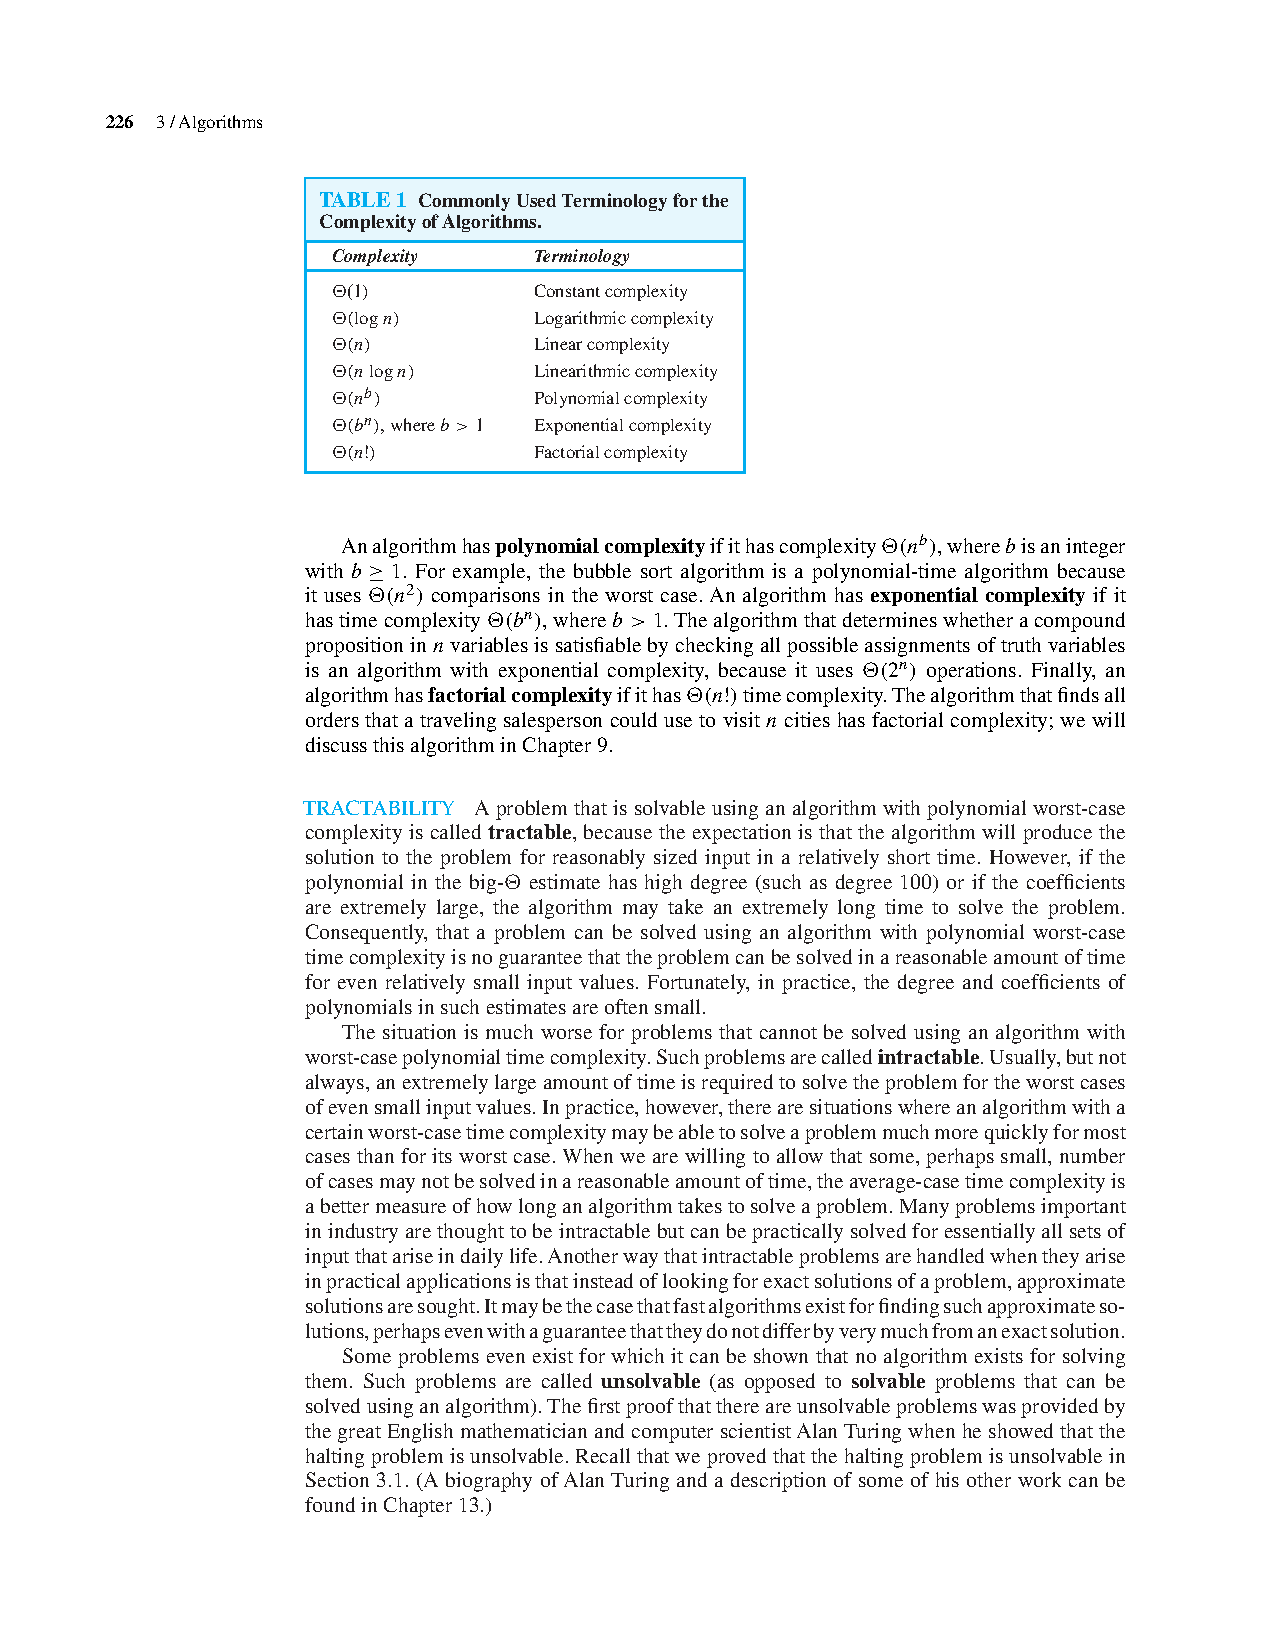
\includegraphics[trim={2cm 19cm 6cm 3cm},clip,width=\linewidth]{p226}
\end{frame}

\begin{frame}{Example 1}
    \begin{itemize}
     \item Give a big-$\mathcal{O}$ estimate for the number of operations (where an operation is an addition or a multiplication) used in this segment of an algorithm.
    \end{itemize}

    \centering 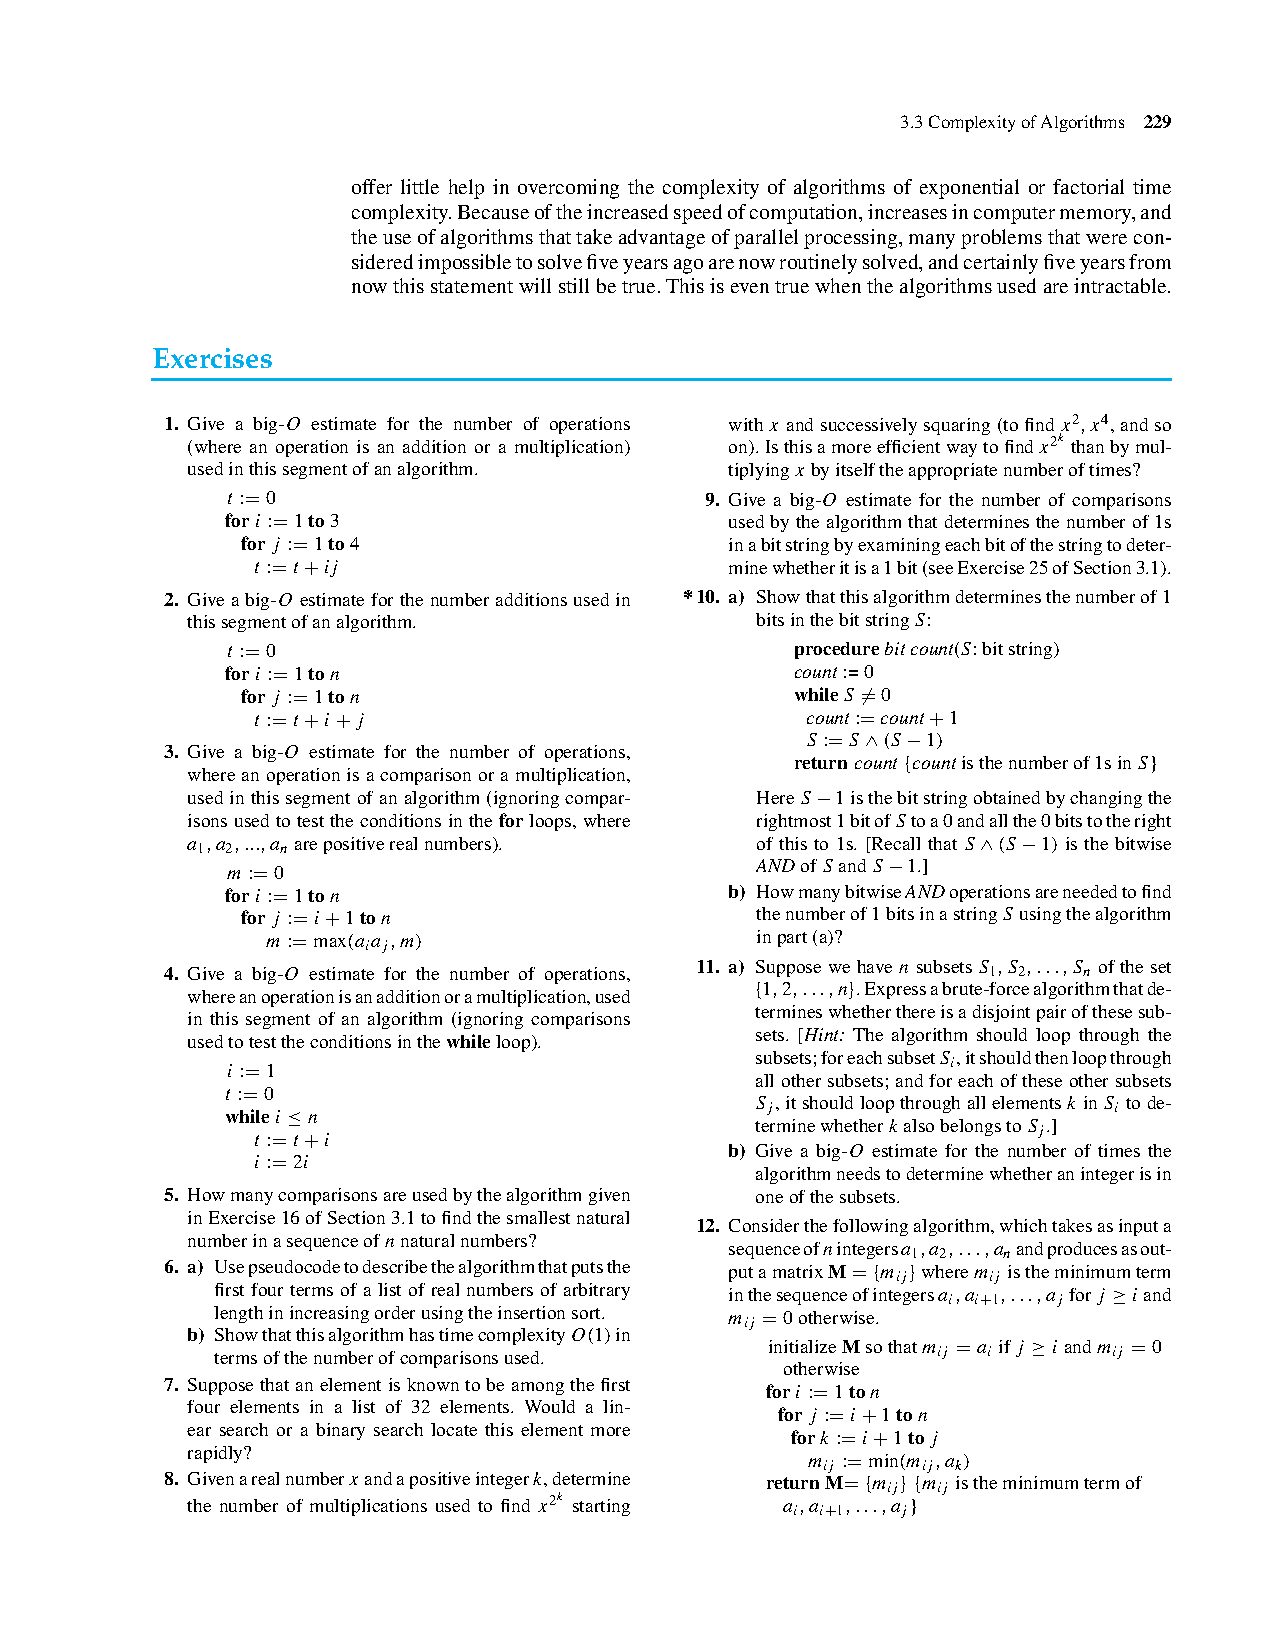
\includegraphics[trim={3cm 18cm 15cm 8.2cm},clip,width=0.4\linewidth]{p229}
\end{frame}

\begin{frame}{Example 1}
    \begin{itemize}
     \item The statement \textbf{t := t + ij} is executed just 12 times, so the number of operations is $\mathcal{O}(1)$. (Specifically, thereare just 24 additions or multiplications.)
    \end{itemize}

    \centering 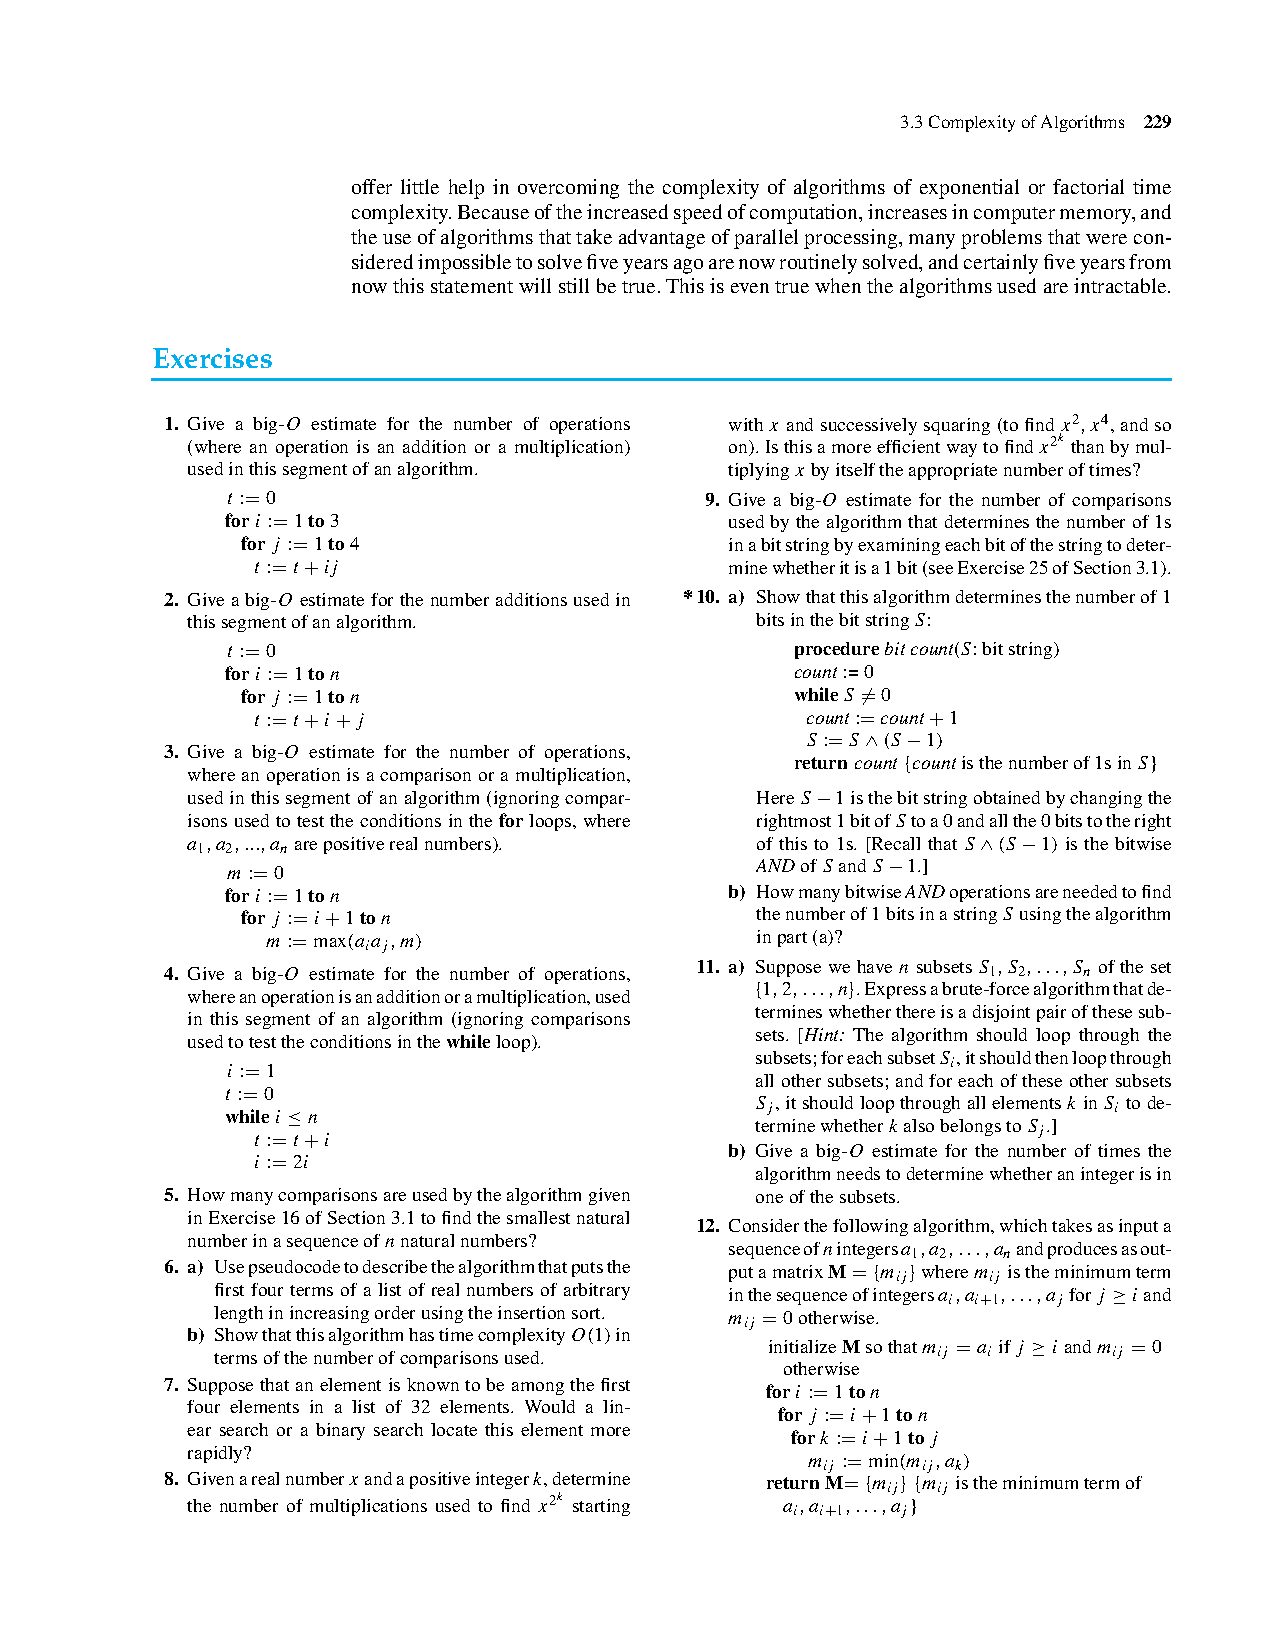
\includegraphics[trim={3cm 18cm 15cm 8.2cm},clip,width=0.4\linewidth]{p229}
\end{frame}

\begin{frame}{Example 2}
    \begin{itemize}
     \item Give a big-$\mathcal{O}$ estimate the number of operations, where an operation is a comparison or a multiplication, used in this segment of an algorithm (ignoring comparisons used to test the conditions in the for loops, where $a_1, a_2, \ldots, a_n$ are positive real numbers).
    \end{itemize}

    \centering 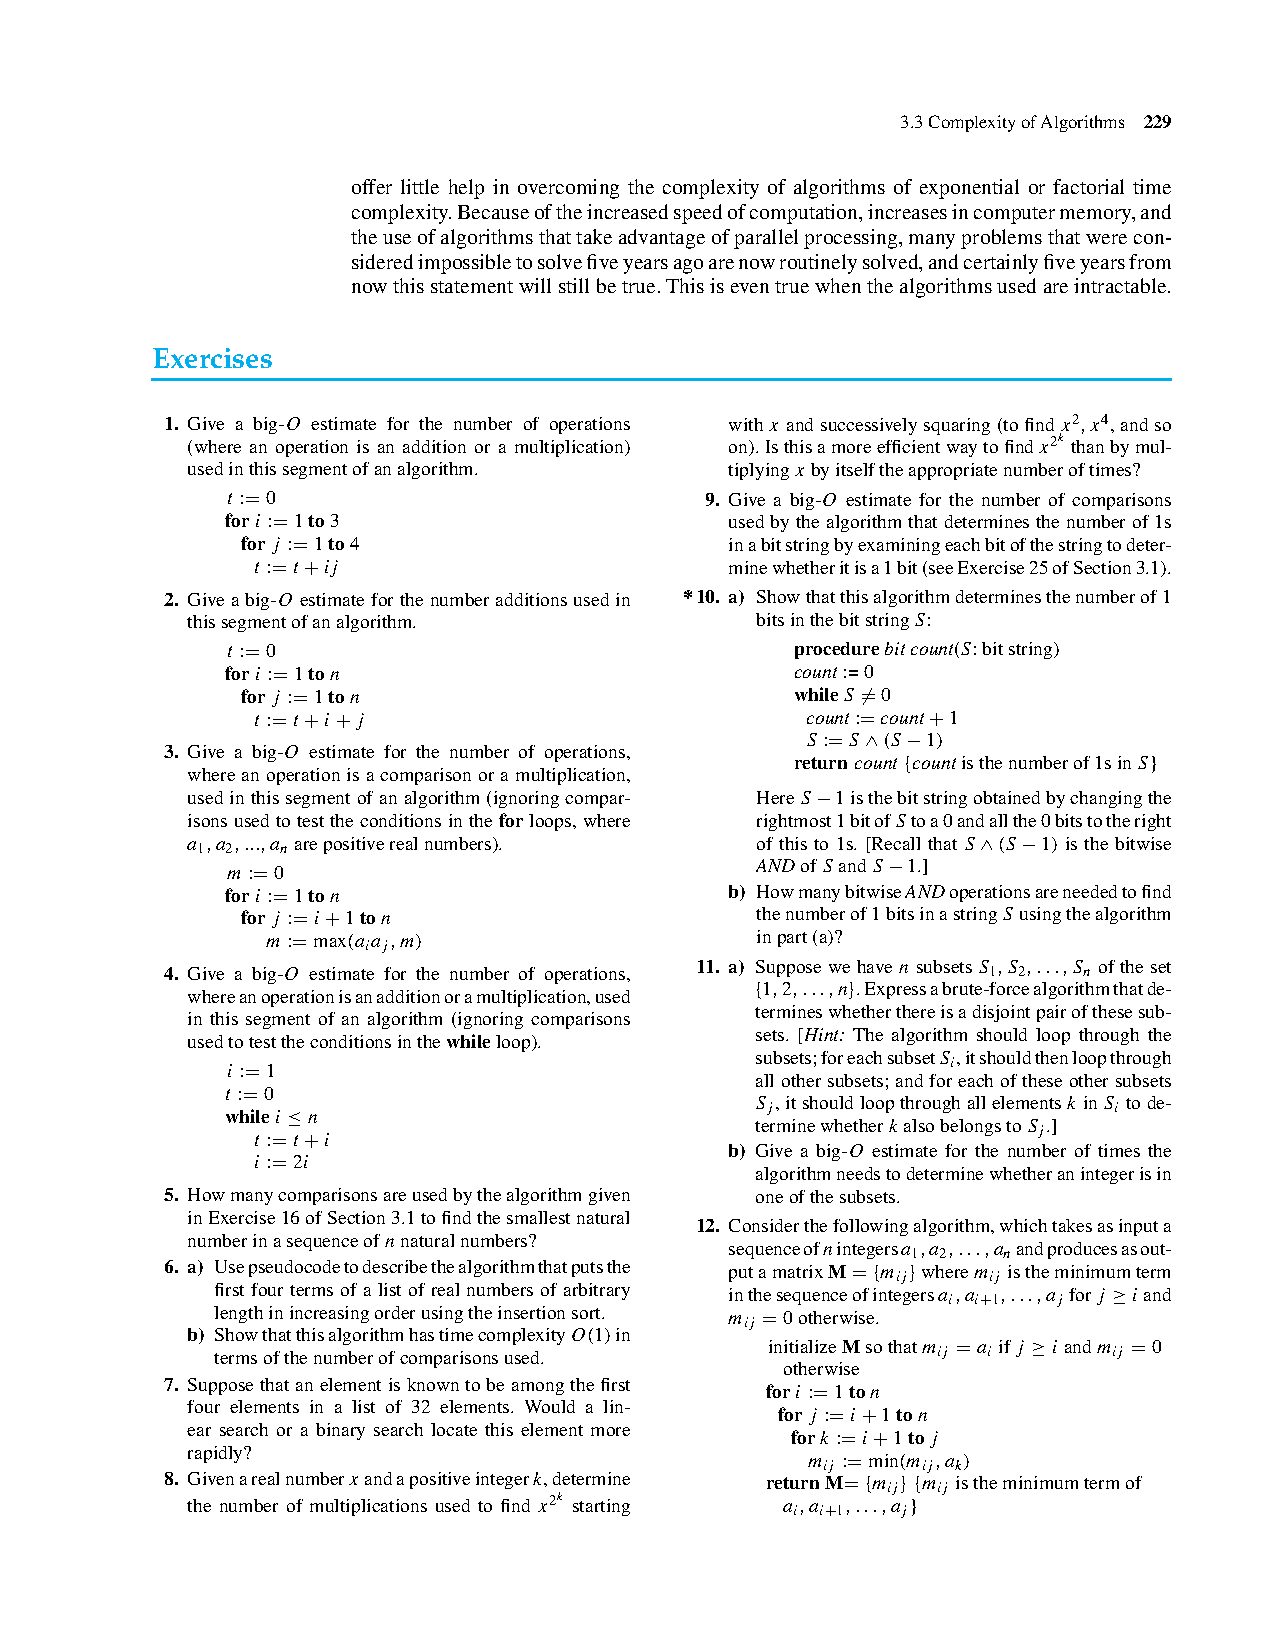
\includegraphics[trim={3cm 11.7cm 14.3cm 14.5cm},clip,width=0.45\linewidth]{p229}
\end{frame}

\begin{frame}{Example 2}
    \begin{itemize}
     \item The nesting of the loops implies that the assignment statement is executed roughly $\frac{n^2}{2}$ times. Therefore the number of operations is $\mathcal{O}(n^2)$.

    \end{itemize}

    \centering 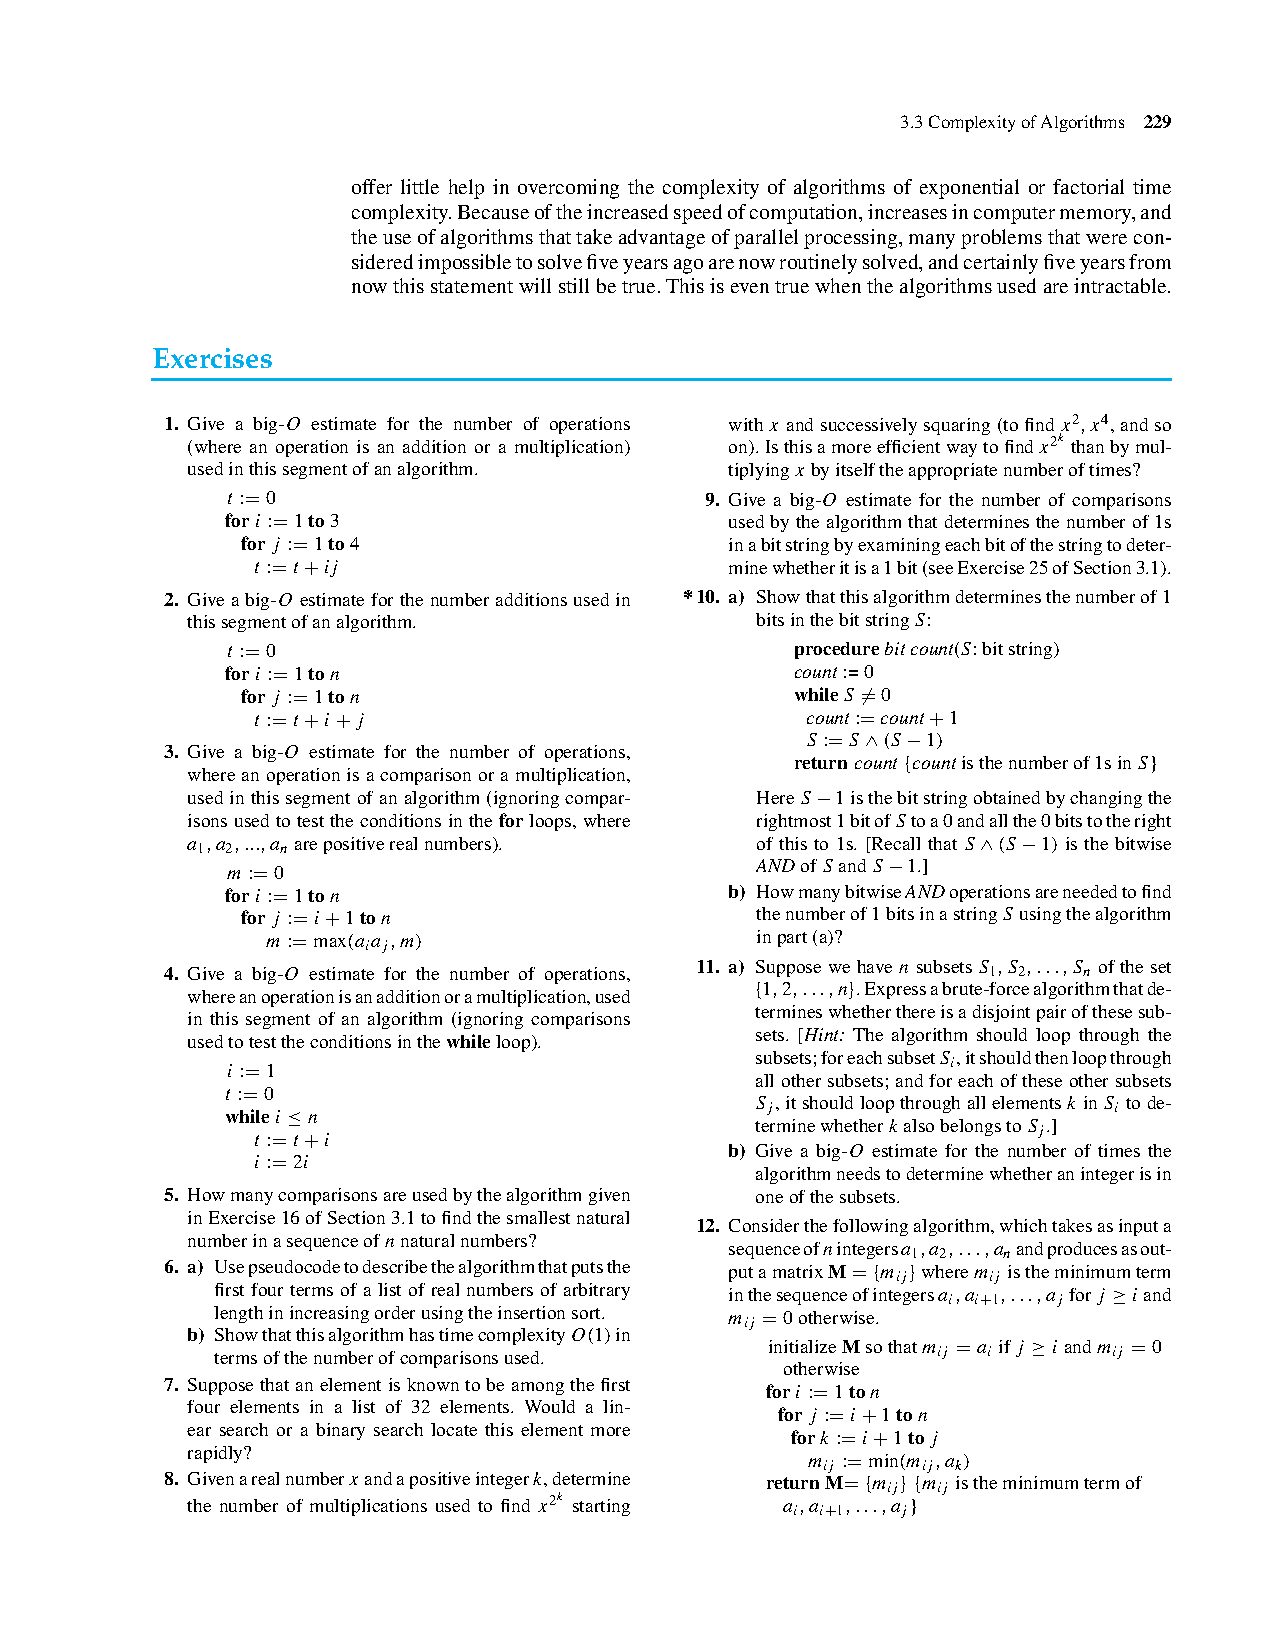
\includegraphics[trim={3cm 11.7cm 14.3cm 14.5cm},clip,width=0.45\linewidth]{p229}
\end{frame}

\begin{frame}{Example 3}
    \centering 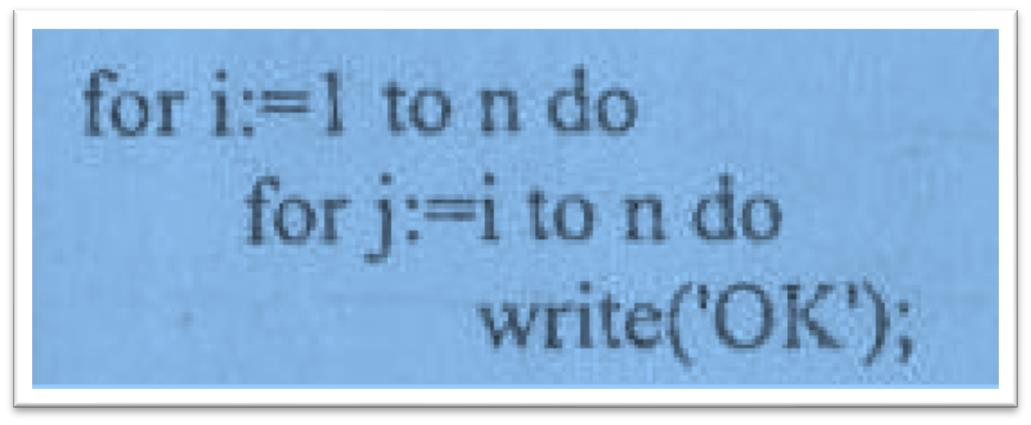
\includegraphics[width=0.45\linewidth]{code}
    \begin{itemize}
     \item $\frac{n(n+1)}{2}$
     \item $\mathcal{O}(n^2)$
    \end{itemize}
\end{frame}

\section*{Reference}

\begin{frame}{Reference}
    \begin{itemize}
        \item Discrete Mathematics and Its Applications. Rosen, K.H. 2012. McGraw-Hill. \\
        Appendix 2: Exponential and Logarithmic functions. \\
        Chapter 3: Algorithms. \\
        Section 3.2: The Growth of Functions. \\
        Section 3.3: Complexity of Algorithms.
    \end{itemize}
\end{frame}

\end{document}
